% Closed-loop timeline of the base experiment, as logged in the run.
\documentclass[border=2pt]{standalone}
\usepackage{tikz}
\usetikzlibrary{arrows.meta}
\begin{document}
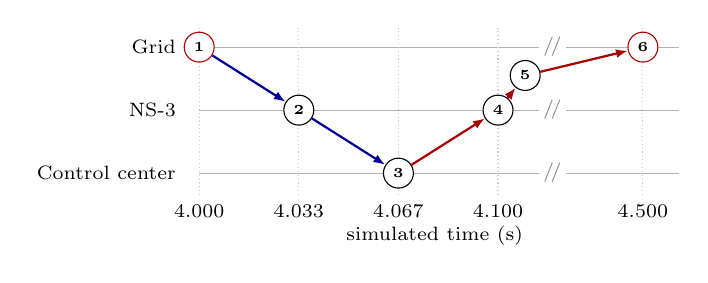
\begin{tikzpicture}[font=\scriptsize, x=1.15cm, y=0.8cm,
  ev/.style={circle, draw, fill=white, inner sep=0.8pt, font=\tiny\bfseries, minimum size=3.8mm},
  arr/.style={-{Latex[length=1.5mm]}, thick}]
\foreach \y/\n in {2/Grid, 1/NS-3, 0/Control center} { \node[anchor=east] at (-0.15,\y) {\n}; \draw[gray!60] (0,\y) -- (3.75,\y); \draw[gray!60] (4.05,\y) -- (5.3,\y); }
\foreach \y in {2,1,0} { \node[gray] at (3.9,\y) {/\!/}; }
\foreach \x/\l in {0/4.000, 1.1/4.033, 2.2/4.067, 3.3/4.100, 4.9/4.500} { \draw[gray!40, densely dotted] (\x,-0.35) -- (\x,2.3); \node[anchor=north] at (\x,-0.35) {\l}; }
\node[ev, draw=red!70!black] (e1) at (0,2) {1};
\node[ev] (e2) at (1.1,1) {2};
\node[ev] (e3) at (2.2,0) {3};
\node[ev] (e4) at (3.3,1) {4};
\node[ev] (e5) at (3.6,1.55) {5};
\node[ev, draw=red!70!black] (e6) at (4.9,2) {6};
\draw[arr, blue!60!black] (e1) -- (e2);
\draw[arr, blue!60!black] (e2) -- (e3);
\draw[arr, red!65!black] (e3) -- (e4);
\draw[arr, red!65!black] (e4) -- (e5);
\draw[arr, red!65!black] (e5) -- (e6);
\node at (2.6,-1.0) {simulated time (s)};
\end{tikzpicture}
\end{document}
